

\newcommand{\onum}[1]{\overline{{#1}}} 	%upper limit interval
\newcommand{\unum}[1]{\underline{{#1}}}  	%lower limit interval

\chapter{Algorithm 1 - Intersection with Interval limits}
% \todo[inline]{David et Vincent: Je vous propose à utiliser les commentaires "tab review" pour gérer les changements un peu plus simplement}
%%%%%%%%%%%%%%%%%%%%%%%%%%%%%%%%%%%%%%%%%%%%%%%%%%%%%%%%%%%%%%%%%%%%%%%%%%%%%%%%

Ellipsoid-based manipulability measures are often used to characterize the force/velocity task-space capabilities of robots. While computationally simple, this approach largely approximates and underestimates the true capabilities. Force/velocity polytopes appear to be a more appropriate representation to characterize the robot's task-space capabilities. However, due to the computational complexity of the associated vertex search problem, the polytope approach is mostly restricted to  offline use, \textit{e.g.} as a tool aiding robot mechanical design, robot placement in work-space and offline trajectory planning. In this paper, a novel on-line polytope vertex search algorithm is proposed. It exploits the parallelotope geometry of actuator constraints. The proposed algorithm significantly reduces the complexity and computation time of the vertex search problem in comparison to commonly used algorithms. In order to highlight the on-line capability of the proposed algorithm and its potential for robot control, a challenging experiment with two collaborating \textit{Franka Emika Panda} robots, carrying a load of 12 kilograms, is proposed. In this experiment, the load distribution is adapted on-line, as a function of the configuration dependant task-space force capability of each robot, in order to avoid, as much as possible, the saturation of their capacity.
% The algorithm execution time for 7DOF \textit{Franka Amika Panda} and for 6DOF \textit{Universal Robots UR5} robots is under 3 and 2 milliseconds respectively.


%%%%%%%%%%%%%%%%%%%%%%%%%%%%%%%%%%%%%%%%%%%%%%%%%%%%%%%%%%%%%%%%%%%%%%%%%%%%%%%%
\section{Introduction}

\begin{figure}[!h]
    \centering
        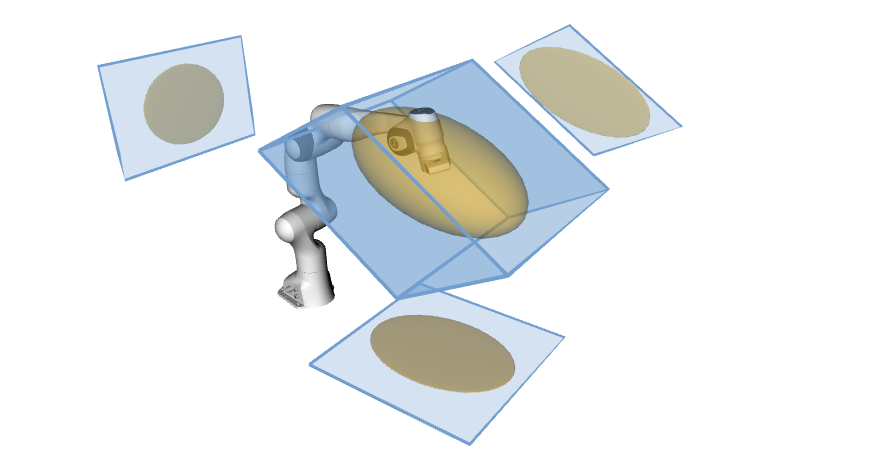
\includegraphics[width=0.8\linewidth]{Papers/images/polytope_ellipsoid.png}
    \caption{2D and 3D force polytopes and their ellipsoid counterparts for a 7 degrees of freedom (DoF) \textit{Franka Emika Panda} robot. Both polytopes and ellipsoids are calculated separately for the 3D and for each of the 2D reduced task-space cases. Both polytopes and ellipsoids take in consideration the true joint torque limits provided by the manufacturer. The underestimation of the true force capabilities of the robot by ellipsoids appears clearly.}

    \label{fig:polytope_ellipsoid}
    \vspace*{-0.3cm}
\end{figure}

Robotics manipulators and their environments are traditionally optimised for a set of specific tasks and their efficiency is based on long-term task execution. Recently, with the introduction of collaborative robots in human environments, robots need to be adaptable to unexpected events, flexible in both task definition and execution and provide high degree of safety for all humans involved. Therefore, evaluating robot capabilities and optimising their performance in advance, with tools designed for more traditional robots, is no longer a suitable approach. New on-line capable and accurate evaluation techniques are needed to account for constantly changing environments, flexible tasks and interaction requirements of collaborative robots.

There are several types of metrics developed to characterise robot's kinematic, kineto-static and dynamic capabilities. The characteristics of robots are related to their kinematics, mechanical design and actuation/joint limits. Kineto-static capabilities of robots characterize the ranges of achievable twists and wrenches in arbitrary directions while in \textit{static conservative conditions}\cite{angeles_design_2016}. Dynamic capabilities characterise ranges of achievable accelerations and link elastic deformations. 

Arguably the most widely used metrics are kineto-static capacity metrics based on \textit{dexterity indices}, expressing robot's ability to move and apply forces and torques in arbitrary directions with equal ease \cite{angeles_design_2016}. The widely used implementation of this metric are velocity and force manipulability ellipsoids, introduced by Yoshikawa \cite{yoshikawa_manipulability_1985}. 
On the one hand, velocity manipulability ellipsoids are often used as a performance measure to optimise robot trajectories and avoid unwanted configurations. On the other hand, force manipulability ellipsoid characterises the forces the robot can apply or resist based on its kinematics. It is used during the design stage of robotic manipulators \cite{angeles_design_2016} as well as for off-line trajectory planning \cite{kuffner_motion_2016} or for on-line control adaptation \cite{joseph2019online}.

Even though manipulability ellipsoids are widely used (mostly because of their calculation efficiency), they are just an approximation and can lead to a drastic underestimation of the real kineto-static capacities of robots \cite{merlet_jacobian_2006}. In the context of collaborative robotics, the margin between the actuation capabilities of the robot and the requirement of the task is largely reduced with respect to more classical, oversized, industrial robots. Thus, any over/under-estimation of the true capabilities of the system has strong negative implications either in terms or safety or in terms of efficiency.

Chiacchio et al.\cite{chiacchio_evaluation_1996} demonstrated that the exact wrench and twist capacities have the form of polytopes. Polytopes do not underestimate the robot capacity \cite{finotello_computation_1998}, can easily integrate variable and non-symmetric limits, dynamics and external forces \cite{merlet_jacobian_2006}. Additionally, in the context of collaborative robotics, when evaluating capacities of multiple robots, sum and intersection of ellipsoids becomes a complex problem to solve and interpret \cite{lee_dual_1989}\cite{chiacchio_task_1991}\cite{julio_frantz_analysis_2015} whereas these operations are well-defined for polytopes. Figure~\ref{fig:polytope_ellipsoid} illustrates the difference of force capability estimation between polytope and ellipsoid characterization.
%Furthermore, since the ellipsoids are considerable underestimation of robot capacities it is certainly important to question the energy efficiency and safety implications.
However, evaluating twist and wrench polytopes relies on a \textit{vertex enumeration} problem \cite{avis_pivoting_nodate} which is a computationally intensive task and is the main obstacle for wider uses of polytopes instead of ellipsoids in practice. 

In this paper, a brief overview of polytope-based task-space capability characterization is given in section~\ref{sec:section_rappel}. Then, a new on-line capable polytope vertex finding algorithm for efficiently calculating twist and wrench polytopes is proposed and described in section~\ref{sec:algorithm}. The new algorithm is capable of calculating polytope vertices for 6DoF and 7DoF robots under 3ms in Python as illustrated in section~\ref{sec:results}. This opens many doors in terms of on-line usage of such capability indicators. To demonstrate the benefits of our method for on-line robot control, an experimental setup with two collaborating \textit{Franka Emika Panda} robots is proposed. It is shown that by leveraging the real carrying capacity on-line measure of the robots, it is possible to design a control strategy allowing to carry, a voluntarily exaggerated, mass of 12 kilograms.  Discussions on the potential applications of the results of this work in collaborative robotics are then proposed in section~\ref{sec:discussion}.


\section{Task-space twist and wrench feasibility polytopes basics}
\label{sec:section_rappel}
For a serial robotic manipulator with $n$ degrees of freedom, with joint space generalized coordinates $\bm{q} \in \mathbb{R}^{n}$ and with Jacobian matrix $J(\bm{q})\in \mathbb{R}^{m \times n}$ (with $m=6$ in the 3D case and $m=3$ in the planar one), the task space Cartesian twist  $\bm{v}$ can be calculated from generalized velocities $\bm{\dot{q}}$ using
\begin{equation}
    \bm{v} = J(\bm{q})\bm{\dot{q}}
    \label{eq:velocity}
\end{equation}
The dual relation relaying the Cartesian wrench $\bm{f} \in \mathbb{R}^m$ with the generalized forces $\bm{\tau} \in \mathbb{R}^n$ is given by
\begin{equation}
    J(\bm{q})^T \bm{f} + \bm{\tau}_0 = \bm{\tau}
    \label{eq:force}
\end{equation}
$\bm{\tau}_0$ is a generalized force that does not ``produce'' any task space wrench, \texit{i.e.} $\bm{\tau}_0$ belongs\footnote{We recall here that $\mathcal{K}er(J(\bm{q})) = \mathcal{I}m(J(\bm{q})^T)^\bot$.} to the kernel $\mathcal{K}er(J(\bm{q}))$ of $J(\bm{q})$. Conversely, $(\bm{\tau}-\bm{\tau}_0)$ lies in the image  $\mathcal{I}m(J(\bm{q})^T)$ of  $J(\bm{q})^T$, \textit{i.e.} ``produces'' task space wrenches.

While equations (\ref{eq:velocity}) and (\ref{eq:force}) describe the kineto-static behaviour of a robot, generalized forces $\bm{\tau}$ and velocities $\bm{\dot{q}}$ are constrained due to the physical limits of the robot construction and actuators
\begin{subequations}
\begin{align}
    \unum{\dot{q}}_{i} \leq & \dot{q}_i \leq \onum{\dot{q}}_{i} \label{eq:constraints_v}\\
    \unum{\tau}_{i} \leq &\tau_i \leq \onum{\tau}_{i}  \label{eq:constraints_f}
\end{align}   
\label{eq:constraints}
\end{subequations}
Given these constraints, the feasible twist polytope defined by equation (\ref{eq:velocity}) can be written
\begin{equation}
\begin{split}
    \mathcal{P}_v = & \left\{ \bm{v} \in \mathbb{R}^{m} \,\big| \, \bm{\dot{q}} \in [ \bm{\unum{\dot{q}}}, \bm{\onum{\dot{q}}} ],~\bm{v} = J(\bm{q})\bm{\dot{q}} \right\}
    \label{eq:polytope_v}
\end{split}
\end{equation}

Similarly, the feasible wrench polytope is defined as\footnote{The dependence of $J$ to $\bm{q}$ is dropped here and when further needed for the sake of clarity.}
% \begin{equation}
%   \mathcal{P}_f = \big\{ \bm{f} \in \mathbb{R}^{m} \,| \, \bm{\tau}_{min} \leq \bm{\tau} \leq \bm{\tau}_{max},\quad \bm{f} = J(\bm{q})^{-T} \bm{\tau} \big\}
%  \label{eq:polytope}
% \end{equation}
% where $J(\bm{q})^{-T}$ inverse of the the transposed jacobian matrix. Above  force polytope $\mathcal{P}_f$ formulation is valid only for non-redundant manipulators, where jacobian matrix in invertable. For redundant manipulators a right \textit{pseudo-inverse} $J(\bm{q})^{T+}$  \cite{klema_singular_1980} of matrix $J(\bm{q})^T$ needs to be calculated and the joint torque vector $\tau$ needs to belong to the image of $J(\bm{q})^T$ matrix \cite{chiacchio_evaluation_1996}.

\begin{equation}
\begin{split}
   \mathcal{P}_f = & \left\{ \bm{f} \in \mathbb{R}^{m}\,\big| \bm{\tau} \in \left\{[\bm{\unum{\tau}},\bm{\onum{\tau}}] \cap \mathcal{I}m(J^T)\right\},J^{T}\bm{f}=\bm{\tau} \right\}
 \label{eq:polytope_f}
\end{split}
\end{equation}


%\todo[inline]{not sure should I explain that we cannot put anything in $\tau$ vector and project it to $f$}

\begin{figure}[!t]
    \centering
    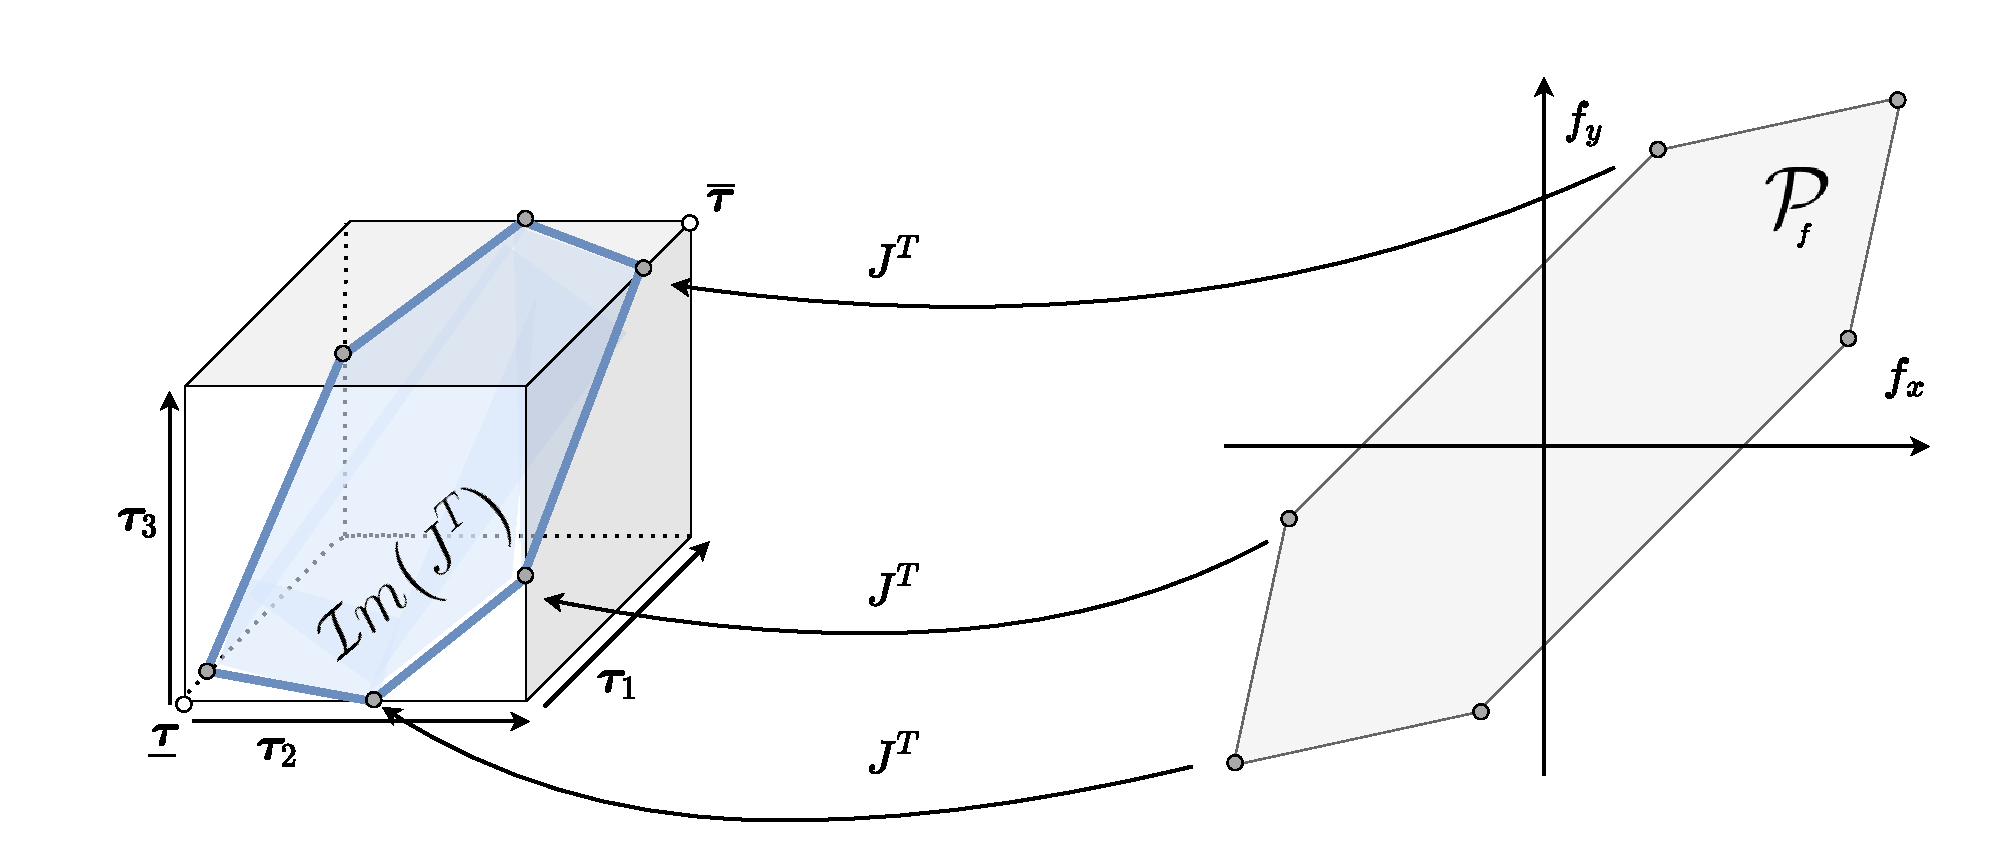
\includegraphics[width=\linewidth]{Papers/images/polytope_search.pdf}
    \caption{Example representation of force polytope $\mathcal{P}_f$ vertices in joint and task-space for a redundant 3DoF planar robot: $n$=$3$, $m$=$2$. }
    \label{fig:polytope_search}
\end{figure}

Equations (\ref{eq:polytope_v}) and (\ref{eq:polytope_f}) provide compact yet implicit representations of the feasible twist and wrench polytope of a robot. The characterization of these capabilities require an explicit definition of these polytopes, \textit{i.e.} a computation of their vertices. In the case of $\mathcal{P}_v$, computing the vertices boils down to determining the convex-hull of the image of the vertices of the constraints polytope defined by equation~(\ref{eq:constraints_v}) through the linear mapping $J(\bm{q})$. The case of $\mathcal{P}_f$ yields an extra difficulty as one first needs to determine the intersection between the constraints polytope defined by equation~(\ref{eq:constraints_f}) and $\mathcal{I}m(J(\bm{q})^T)$.

Over the years many vertex search (enumeration) methods have been proposed \cite{avis_comparative_2015}. Most of the approaches in literature are optimised to solve high dimensional problems and provide an abstraction from the actual system that is being analysed. One of the most commonly used method for vertex enumeration is the double description method \cite{avis_pivoting_nodate} which formulates the vertex search problem as transformation of a half-space representation $\mathcal{H}-rep$ to a vertex representation $\mathcal{V}-rep$. This formulation generalizes well in between different high dimensional problems but lacks the flexibility to incorporate information about the physical system being analysed. 

Therefore, various methods have been introduced in order to leverage specific problem formulation and improve the computational performance of vertex search. The scaling factor method has been developed for planar parallel robots \cite{nokleby_force_2005} and later adapted to planar serial manipulators \cite{julio_frantz_analysis_2015}. This method reduces the search space with one scaling factor to an exhaustive search in the scalar space. A very efficient algorithm for planar robots has also been proposed by Gouttefarde et al. \cite{gouttefarde_versatile_2015} which navigates the polytope boundaries in search for extremities. Both the scaling factor and boundaries navigation methods are designed for planar vertex search and do not scale to three dimensional world.

Chiacchio et al. in their original paper \cite{chiacchio_evaluation_1996} propose an algorithm for finding the vertices of task-space polytopes by introducing slack variables and performing an exhaustive search through the joint space limits. This algorithm, although significantly improving the evaluation still remains too complex for on-line execution. This algorithm has been improved by Sasaki et al. \cite{sasaki_vertex_nodate} where the computational complexity has been significantly reduced by introducing the geometrical representation of actuator constraints as an $n$-dimensional parallelotope.

The next section introduces additional improvements of the algorithms proposed in \cite{chiacchio_evaluation_1996} and \cite{sasaki_vertex_nodate}. The resulting algorithm significantly reduces the computation time and complexity of the vertex enumeration problem for task-space polytopes. The proposed description is restricted to the most complex case of $\mathcal{P}_f$ but the method is also computationally beneficial in the simpler case of computing $\mathcal{P}_v$. Also in order to ease illustrations, the considered task-space wrench is limited to its force component without any loss of generality.

\section{Vertex finding algorithm formulation}
\label{sec:algorithm}
%\todo[inline]{
% \begin{itemize}
%     \item introduce the new algorithm
%     \item pseudocode maybe
%     \item nice figure
%     \item explain the check before inversion
% \end{itemize}
% }

For an $n$DoF serial manipulator, the feasible space of joint torques $\bm{\tau}$ forms an $n$-dimensional parallelotope with $n$ pairs of parallel faces defined by the joint limits (\ref{eq:constraints_f}). The image of the Jacobian transpose matrix $\mathcal{I}m(J(\bm{q})^T)$ is a $r$-dimensional subspace of the parallelotope (where $r$ is the rank of $J(\bm{q})^T$ and $r$=$m$ for non-singular configurations\footnote{In the remainder of this paper, the robot is, without loss of generality, assumed to be in a non singular configuration.}), which corresponds to set of torques yielding non zero task space wrenches. 
Sasaki et al. \cite{sasaki_vertex_nodate} have shown that the extreme values of joint torques $\bm{\tau_{vert}} \in \mathcal{I}m(J(\bm{q})^T)$ belong to the $n$-$m$ dimensional faces of the constraint parallelotope.  Furthermore, there is a one-to-one correspondence between $\bm{\tau_{vert}}$ torque vertices and the $\bm{f}_{vert}$ vertices of polytope $\mathcal{P}_f$ can be computed as 
\begin{equation}
    \bm{f}_{vert} = J(\bm{q})^{T+}\bm{\tau}_{vert} \label{eq:compute_vert}
\end{equation}
where $J(\bm{q})^{T+}$ is the pseudo-inverse of $J(\bm{q})^{T}$ which provides the unique and exact solution of the inversion problem in this specific case.

Figure \ref{fig:polytope_search} shows the example of a 3DoF planar robot ($n$=$3$, $m$=$2$) for which the joint torque space is a cube and $\mathcal{I}m(J(\bm{q})^T)$ is a plane. The extreme values of feasible joint torques are found on its $n-m=1$ dimensional faces, \textit{i.e} its edges. For the example shown in figure \ref{fig:intersection_example}, $n$=$3$ and $m$=$1$ so the vertices belong to the $n-m=2$ dimensional faces of the cube, \textit{i.e.} its 2D sides.  

Therefore, state-of-the-art algorithms such as \cite{chiacchio_evaluation_1996} and \cite{sasaki_vertex_nodate} propose an exhaustive search over all the $n$-$m$ dimensional parallelotope faces to find the extreme values of joint torques $\bm{\tau_{vert}}$ and consequently the vertices of force polytope $\mathcal{P}_f$. In this paper, a new representation of joint torque vector $\bm{\tau}$ is proposed enabling an efficient navigation of the $n-m$ dimensional parallelotope faces, reducing the complexity of the exhaustive search.

\subsection{Proposed algorithm}

Consider a joint torque vector $\bm{\tau}$ meeting constraints~\ref{eq:constraints_f}. It can be defined as
\begin{equation}
    \bm{\tau} = \unum{\bm{\tau}} + \alpha_1 \bm{\tau}_1+ \alpha_2 \bm{\tau}_2 + ... + \alpha_n \bm{\tau}_n
    \label{eq:torque_new}
\end{equation}
where $\alpha_i \in [0,1]$ are scalars weights and vectors $\bm{\tau}_i$ are orthogonal base vectors in joint space aligned with $i$-th axis of the parallelotope, defined as $\bm{\tau}_i = \begin{bmatrix} 0~\ldots~\onum{\tau}_{i} - \unum{\tau}_{i}~\ldots~0 \end{bmatrix}^T$. 

Since the vertices $\bm{\tau_{vert}} \in \mathcal{I}m(J(\bm{q})^T)$ belong to the $n$-$m$ dimensional faces of the joint torque parallelotope, representation (\ref{eq:torque_new}) provides an elegant way to navigate them, by fixing $m$ out of $n$ scalars $\alpha_i$ either to $0$ or to $1$.

\begin{figure}[!t]
    \centering
    \hspace*{-0.5cm}
    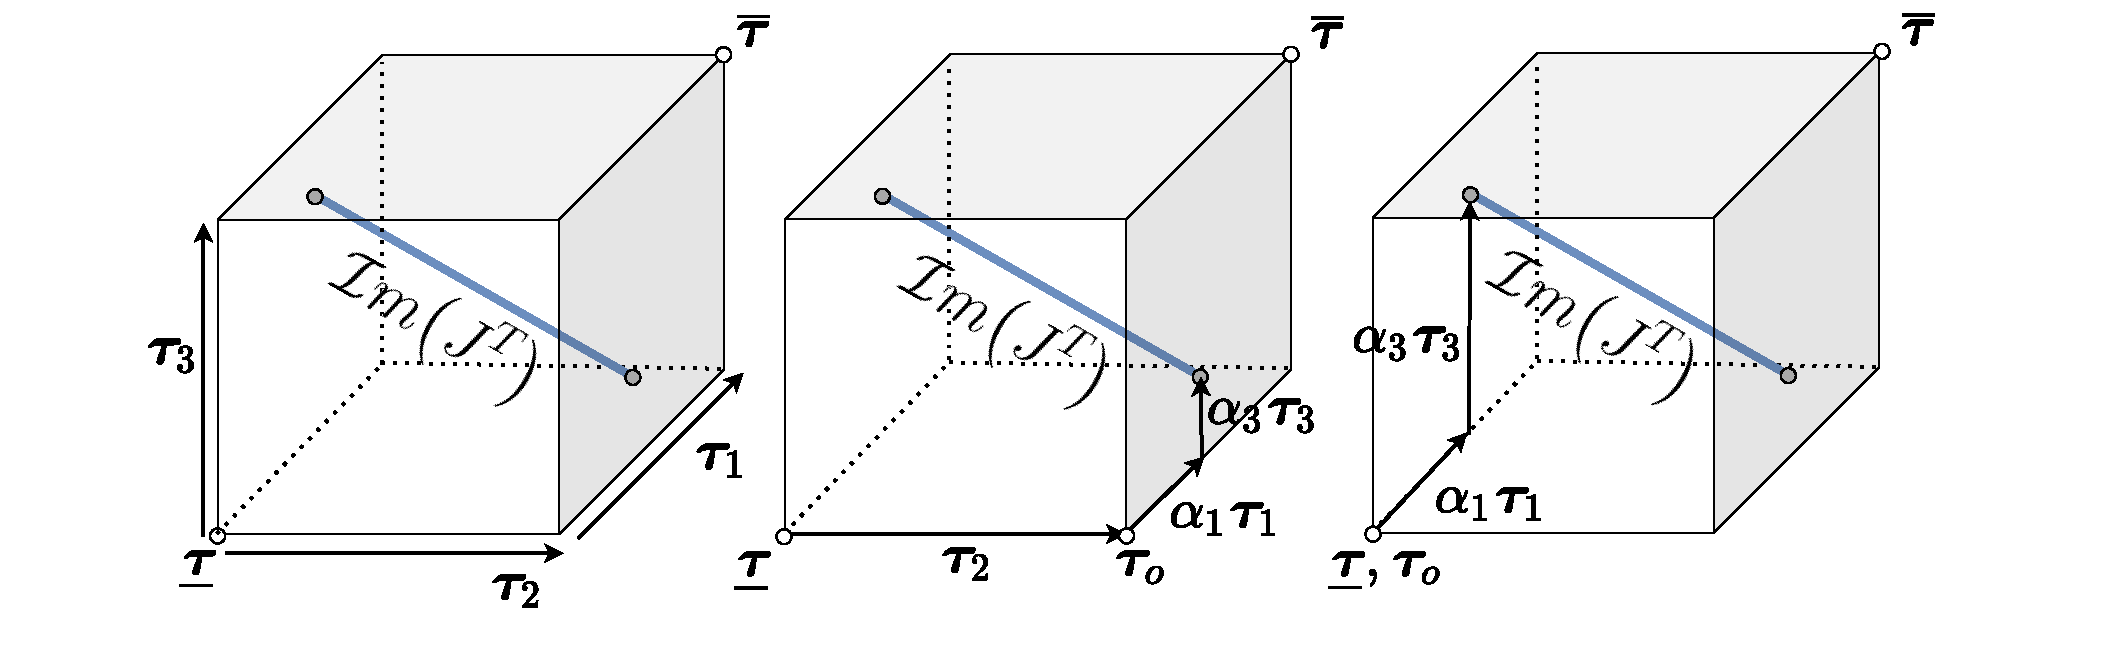
\includegraphics[width=1.1\linewidth]{Papers/images/intersection_example.pdf}
    \caption{Example of joint space interpretation of the vertex search algorithm solution for $n$=$3$ and $m$=$1$. }
    \label{fig:intersection_example}
    \vspace*{-0.3cm}
\end{figure}

An $n$-dimensional parallelotope has $\big(\begin{smallmatrix}n\\m\end{smallmatrix}\big)$ sets of $2^m$ parallel $n$-$m$ dimensional faces. Each set of parallel faces can be represented with the linear combination of the same set of $n$-$m$ base vectors $\bm{\tau}_i$ or in other words with a set of $n$-$m$ scalars $\alpha_i$. The remaining $m$ scalars are set either to 0 or 1 and define the origin $\bm{\tau}_o$ of  each one of the $2^m$ faces from the set
\begin{equation}
    \bm{\tau}_o = \unum{\bm{\tau}} + \alpha_1 \bm{\tau}_1+ ... + \alpha_m \bm{\tau}_m
\end{equation} 
Therefore, each $n$-$m$ dimensional face can be reached by partitioning $\bm{\alpha} = \left[\bm{\alpha}_1^T ~\bm{\alpha}_2^T\right]^T$, $\bm{\alpha}_1$ containing $m$ scalars $\alpha_i$ fixed to $0$ or $1$ and $\bm{\alpha}_2$ containing the remaining $n$-$m$ scalars which define the linear combination of $n$-$m$ base vectors $\bm{\tau}_i$.

Figure \ref{fig:intersection_example} illustrates the case where $\mathcal{I}m(J^T)$ is a line in joint space. In this case the intersection space is $n$-$m$=$2$ dimensional. In this case, two scalars $\alpha_1$ and $\alpha_3$ are enough to characterise both vertices of interest with $\alpha_2$ fixed to $0$ or $1$.

In order to find the vertices of the force polytope $\mathcal{P}_f$, equations (\ref{eq:force}) and (\ref{eq:torque_new}) are combined to restrict the search to the set of torques $\bm{\tau} \in \left\{[\bm{\unum{\tau}},\bm{\onum{\tau}}] \cap \mathcal{I}m(J^T)\right\}$
\begin{equation}
    J(\bm{q})^T \bm{f}_{vert} = \unum{\bm{\tau}} + \alpha_1 \bm{\tau}_1+ \alpha_2 \bm{\tau}_2 + ... + \alpha_n \bm{\tau}_n \label{eq:inter_im_bounds_torque}
\end{equation}
For each $\left(\begin{smallmatrix}n\\m\end{smallmatrix}\right)$ combination of the $m$ scalars, $2^m$ values of $\bm{\tau}_o$ can be calculated. For each possible value of $\bm{\tau}_o$, a linear system deriving from equation~(\ref{eq:inter_im_bounds_torque}) can be solved to find the $n$-$m$ scalars $\bm{\alpha}_{2}$ and the corresponding force polytope vertex $\bm{f}_{vert}$
\begin{equation}
    \underbrace{\begin{bmatrix}J(\bm{q})^T&-\bm{\tau}_{m}_{+1} \, \dots \, -\bm{\tau}_{n} \end{bmatrix}}_{Z_{n\times n}} \begin{bmatrix}\bm{f}_{vert}\\ \alpha_{m+1} \\ \vdots\\\alpha_{n} \end{bmatrix} = \bm{\tau}_o
    \label{eq:linear_system_full}
\end{equation}
If $Z$ is invertible and if $\bm{\alpha}_2 \in [\bm{0},\bm{1}]$, $\bm{f}_{vert}$ is a vertex of the polytope $\mathcal{P}_f$
\begin{equation}
   \begin{bmatrix}\bm{f}_{vert}\\ \bm{\alpha}_{2} \end{bmatrix} = Z^{-1}\bm{\tau}_L, \quad  \bm{\alpha}_{2} \in [\bm{0},\bm{1}]
    \label{eq:linear_system_full_solution}
\end{equation}

Overall, in order to navigate all possible combinations of the $n$-$m$ dimensional faces which may contain vertices of the force polytope $\mathcal{P}_f$, $\big(\begin{smallmatrix}n\\m\end{smallmatrix}\big)$=$\frac{n!}{m!(n-m)!}$ inversions of $Z$ and  $2^m \frac{n!}{m!(n-m)!}$ checks that $\bm{\alpha}_2 \in [\bm{0},\bm{1}]$ have to be performed.

In the case depicted in figure \ref{fig:intersection_example} ($n$=$3$, $m$=$1$), $Z$ is inverted only $\big(\begin{smallmatrix}3\\1\end{smallmatrix}\big)$=$3$ times and conditions are evaluated 6 times, which exactly corresponds to the number of faces of the parallelotope. Taking the example of the 3DoF planar robot ($n$=$3$, $m$=$2$) the number of $Z$ inversions is 3 and the number of condition evaluation is 12, which exactly corresponds to the number of edges of the parallelotope. One of the nice features of this approach is that it does not require an explicit inversion of $J(\bm{q})^T$ as in equation~(\ref{eq:compute_vert}) to actually obtain the set of vertices composing $\mathcal{P}_f$.  
% \todo[inline]{Insist maybe that with this approach there is no need to do pseudo-inverse of jacobian and we obtain forces directly. An elegant way.}

\subsection{Improvement using the SVD}

In order to further improve the efficiency of the proposed algorithm the Singular Value Decomposition (SVD) \cite{klema_singular_1980} of $J(\bm{q})$ is used
\begin{equation}
     J(\bm{q}) =  U  \underbrace{\begin{bmatrix}S & O_{m\times (n-m)}\end{bmatrix}}_{\Sigma}\underbrace{\begin{bmatrix}V_1^T \\ V_2^T \end{bmatrix}}_{V^T}
\end{equation}
where $S= diag( \sigma_1 \dots \sigma_m)$ is a diagonal matrix containing the $m$ singular values of $J(\bm{q})$. $V_1^T \in \mathbb{R}^{m \times n}$ projects the space of generalized torques onto the preimage of $\mathcal{I}m(J(\bm{q}))$ and $V_2^T \in \mathbb{R}^{n-m \times n}$ is a basis of $\mathcal{K}er(J(\bm{q}))$. $V_1^T$ and $V_2^T$ are orthogonal vector subspaces yielding $V_2^T V_1 = O$ and thus 
% Since image-space and null-space of the jacobian matrix are orthogonal, all the joint torque vectors $J(\bm{q})^T\bm{f}=\bm{\tau}$ that belong to the image-space of the jacobian matrix will have zero projection to the null-space:
\begin{equation}
    V_2^T J(\bm{q})^T\bm{f} = \bm{0}
\end{equation}
This allows to reduce (\ref{eq:linear_system_full}) to
\begin{equation}
    \underbrace{V_2^T\begin{bmatrix}-\bm{\tau}_{m}_{+1} \dots -\bm{\tau}_{n} \end{bmatrix}}_{T_{(n-m)\times (n-m)}} \bm{\alpha}_2 = V_2^T\bm{\tau}_o
    \label{eq:linear_system_svd}
\end{equation}
If $T$ is invertible, $\bm{\alpha}_2$ can be computed by
\begin{equation}
\bm{\alpha}_2 = T^{-1}V_2^T\bm{\tau}_o
\end{equation}
When the computed $\bm{\alpha}_2 \in [\bm{0},\bm{1}]$,  the corresponding force polytope vertex can be calculated as
\begin{equation}
    \bm{f}_{vert} = J(\bm{q})^{T+} \big( \unum{\bm{\tau}} + \alpha_1\bm{\tau}_{1} +\dots+\alpha_n\bm{\tau}_{n}\big)
\end{equation}

This new approach requires the calculation of the SVD and the Jacobian matrix pseudo-inverse $J(\bm{q})^{T+}$. Nevertheless, since the Jacobian transpose pseudo-inverse can be efficiently calculated from the SVD as $J(\bm{q})^{T+} = U\Sigma^{T+}V^T$
and since both the SVD and pseudo-inverse are calculated once and of all per algorithm run, the computation efficiency is greatly improved due to the matrix dimension reduction from $n$ to $(n-m)$ when inverting $T$ instead of $Z$.


\subsection{Matrix inverse condition}

Due to the constrained nature of $\bm{\alpha}_2$, it is possible to efficiently calculate some bounds ${\bm{t}_{ub}}$ and $\bm{t}_{lb}$ such that $T\bm{\alpha}  \in [\bm{t}_{lb}, \bm{t}_{ub}]$.
%, defining the interval of null-space projections of the vector $\bm{\tau}_o$.
These bounds are found by row-wise summing only positive and only negative elements $t_{ij}$ of  $T$
\begin{equation}
t_{i,lb} = \sum_j \max(t_{ij}, 0), \qquad
t_{i,lb} = \sum_j \min(t_{ij}, 0) 
\label{eq:bounds_condition}
\end{equation}

This creates a bounding box around the space defined with the vector $T\bm{\alpha}_2$. Therefore, one can conclude that if all the $2^m$ combinations of $\bm{\tau}_o \notin [\bm{t}_{lb}, \bm{t}_{ub}] $, the system (\ref{eq:linear_system_svd}) cannot have a solution which satisfies $\bm{\alpha}_2 \in [\bm{0},\bm{1}]$, and there is no need to invert $T$ to figure it out.
% \begin{equation}
%     \forall \bm{\tau}_o, \quad s.t.\quad \quad V_2^T\bm{\tau}_o \not\in [\bm{t}_{lb}, \bm{t}_{ub}] 
% \end{equation}

\subsection{Extension to residual polytopes}

When evaluating the capability of a robot, it is a common practice to take into consideration the joint torques necessary to compensate for gravity $\bm{\tau}_g = \bm{g}(\bm{q})$ \cite{wei_output_nodate} 
\begin{equation}
    J(\bm{q})^T \bm{f} = \bm{\tau} - \bm{\tau}_g
\end{equation}
Furthermore, the same can be done to include the effects of the robot dynamics. For a fixed-base, serial manipulator the dynamics can be written as
\begin{equation}
    M(\bm{q})\ddot{\bm{q}} + C(\dot{\bm{q}},\bm{q})\dot{\bm{q}} + \bm{g}(\bm{q}) = \bm{\tau} - J(\bm{q})^T \bm{f}
    \label{eq:full_dynamics}
\end{equation}
where $M$ and $C$ are respectively the mass and Coriolis-Centrifugal matrices. The residual joint torque vector $\bm{\tau}$ can then be expressed as
\begin{equation}
    J(\bm{q})^T \bm{f} = \bm{\tau} - \bm{\tau}_g  - \big(\underbrace{M(\bm{q})\ddot{\bm{q}} + C(\dot{\bm{q}},\bm{q})\dot{\bm{q}}) \big)}_{\bm{\tau}_{d}}
    \label{eq:force_dynamics}
\end{equation}

Finally, in many cases it is useful to evaluate the residual force ability of a robot already applying a certain nominal wrenches $\bm{f}_{n}$ which imply to generate joint torques $\bm{\tau}_{n}$
\begin{equation}
\bm{\tau}_{n} =  J(\bm{q})^T \bm{f}_{n}  
\end{equation}

The \textit{residual force polytope} \cite{ferrolho_residual_2020} corresponding to the  feasible space of Cartesian wrenches $\bm{f}$ that can be applied and rejected by the robot end-effector, taking into consideration the torque necessary to overcome gravity $\bm{\tau}_{g}$, robot dynamics $\bm{\tau}_{d}$ and any nominal joint torque $\bm{\tau}_{n}$, can be computed using algorithm~\ref{alg:main_algo} and the updated joint constraints
\begin{equation}
\begin{split}
    \unum{\bm{\tau}}' &= \unum{\bm{\tau}} - \bm{\tau}_g - \bm{\tau}_{d} - \bm{\tau}_{n}  \\ 
    \onum{\bm{\tau}}' &= \onum{\bm{\tau}}  - \bm{\tau}_g - \bm{\tau}_{d} - \bm{\tau}_{n}
    \label{eq:residual_constraints}
\end{split}
\end{equation}

% To include the influences of the gravity $\bm{\tau}_{g}$, dynamics of movement $\bm{\tau}_{d}$ and applied nominal wrenches $\bm{\tau}_{n}$, the joint constraints (\ref{eq:constraints_f}) become
% \begin{equation}
% \begin{split}
%     \unum{\bm{\tau}}' &= \unum{\bm{\tau}} - \bm{\tau}_g - \bm{\tau}_{d} - \bm{\tau}_{n}  \\ 
%     \onum{\bm{\tau}}' &= \onum{\bm{\tau}}  - \bm{\tau}_g - \bm{\tau}_{d} - \bm{\tau}_{n}
%     \label{eq:residual_constraints}
% \end{split}
% \end{equation}

% The feasible space of Cartesian wrenches $\bm{f}$ that can be applied and rejected by robot end-effector, taking into consideration the torque necessary to overcome gravity $\bm{\tau}_{g}$, robot dynamics $\bm{\tau}_{d}$ and any nominal joint torque $\bm{\tau}_{n}$ is called \textit{residual force polytope} \cite{ferrolho_residual_2020}. 

\begin{algorithm}[!h]
\caption{New vertex search algorithm pseudo-code}
\begin{algorithmic}
\REQUIRE $J$, $\onum{\bm{\tau}}$, $\unum{\bm{\tau}}$ (Eq. \ref{eq:constraints_f} or Eq. \ref{eq:residual_constraints}) 
\STATE $U, \Sigma, V^T \leftarrow svd(J)$ 
\STATE $J^{T+} = U\Sigma^{T+}V^T$
\STATE $V_1,\, V_2  \leftarrow V $
\STATE calculate $n$ base vectors $\bm{\tau}_1 \dotsc \bm{\tau}_n$ (Eq. \ref{eq:torque_new})

\FORALL{  $\big(\begin{smallmatrix}n\\m\end{smallmatrix}\big)$ combinations of $m$ fixed $\alpha_i$ } 
\STATE construct $T$ matrix (Eq. \ref{eq:linear_system_svd})
\STATE find bounds $\bm{t}_{lb},\bm{t}_{ub}$ (Eq. \ref{eq:bounds_condition})

\FORALL{   $2^m$ vectors $\bm{\tau}_o$ } 
\IF{$ V_2^T\bm{\tau}_o \in [\bm{t}_{lb},\bm{t}_{ub}] $}
\STATE $\bm{\alpha}_2 = T^{-1}V_2^T\bm{\tau}_o $
\IF{$ \bm{\alpha}_2 \in [0,1] $}
\STATE $\bm{\tau}_{vert} = \unum{\bm{\tau}} + \alpha_1{\bm{\tau}_{1}} +\dots+\alpha_n{\bm{\tau}_{n}}$
\STATE $\bm{f}_{vert} = J^{T+}\bm{\tau}_{vert}$
\ENDIF
\ENDIF
\ENDFOR
\ENDFOR

\end{algorithmic}
\label{alg:main_algo}
\end{algorithm}

\section{Complexity analysis}\label{sec:complexity}
To demonstrate the efficiency of the proposed polytope vertex search algorithm, it is compared to the polytope vertex search algorithm introduced by Chiacchio et al. \cite{chiacchio_evaluation_1996}. Furthermore the comparison is extended to the algorithm proposed by Sasaki et al. \cite{sasaki_vertex_nodate} which is, to our knowledge, the only algorithm exploiting the geometric structure of the problem.


% \begin{table*}[!b]
%     \centering
%     \caption{Complexity and execution time comparison for three vertex search algorithms in general case, for  4 DOF planar robot, 6DOF and 7DOF collaborative robots}
%     \begin{tabular}{r | r |c | c | c}
%       \toprule
%       \textbf{Robot} & \textbf{Metric} & \textbf{Chiacchio}\cite{chiacchio_evaluation_1996} & \textbf{Sasaki} \cite{sasaki_vertex_nodate}  &  \textbf{Our approach} \\
%       \hline
%       $\smash{n,m}$& matrix inv. & $ \frac{2n!}{m!(2n-m)!}$ & $ \frac{n!}{m!(n-m)!} $ & $ \leq \frac{n!}{m!(n-m)!}$ \\
%       & matrix dim.  & $ 2n \times 2n$ & $ m\times m $ & $n$-$m$ $\times$ $n$-$m$\\
%       & time[ms] & & & \\
%       \hline
%       \textit{4 link} &  matrix inv. & 24 & 6 & 4.2 $\pm$ 1.4 (6) \\ 
%         $n$=$4$&matrix dim.  & 8x8 & 2x2 & 2x2 \\ 
%       $m$=$2$& time[ms] & 2.7 $\pm$ 0.1 (3.6) & 0.93 $\pm$ 0.1 (1.1) & 0.64 $\pm$ 0.1 (1.5) \\ 
%       \hline
%       \textit{UR5} &  matrix inv. & 220 & 20 & 2.8 $\pm$ 2.5 (10) \\ 
%         $n$=$6$&matrix dim.  & 12x12 & 3x3 & 3x3 \\ 
%       $m$=$3$& time[ms] & 14.2 $\pm$ 0.9 (20) & 2.1 $\pm$ 0.2 (3.4) & 1.5 $\pm$ 0.2 (2.7) \\ 
%       \hline
%       \textit{Panda} &   matrix inv.  &  364 & 35 & 7.3 $\pm$ 4.2 (20)\\
%       $n$=$7$ & matrix dim.  &  14x14 & 3x3 & 4x4\\
%       $m$=$3$&time[ms]  &  25 $\pm$ 0.5 (27) & 3.5 $\pm$ 0.1 (5.4) & 2.6 $\pm$ 0.2 (4.3)\\
%       \bottomrule
%     \end{tabular}
%     \label{tab:complexity_results}
% \end{table*}




The three algorithms have been tested to find vertices of the force polytope $\mathcal{P}_f$ for three different robots: a 4R planar robot ($n$=$4$,$m$=$2$), the \textit{Universal Robots} UR5 6DoF robot ($n$=$6$,$m$=$3$) and the \textit{Franka Emika Panda} 7DoF robot ($n$=$7$,$m$=$3$). The results are averaged over 1000 randomly selected robot configurations. All algorithms have been implemented in the programming language Python and tested on a laptop equipped with a 1.90GHz Intel i7-8650U processor. The code of the proposed algorithm is publicly available\footnote{ \url{https://gitlab.inria.fr/askuric/polytope\_vertex\_search}}.

Table \ref{tab:complexity_results} shows the results of this complexity evaluation. The proposed vertex search algorithm drastically reduces the number of matrix inversions and thus reduces the processing time considerably: $4$-$10\times$ faster execution than Chiacchio's algorithm and on average 20\% faster than Sasaki's. Results show that even for the cases of 6DoF and 7DoF industrial robots our approach is capable of evaluating the polytope vertices under $3ms$. Such a low processing time opens numerous opportunities for the on-line use of polytope based capacity evaluation especially in the area of robot control.

\begin{table}
    \centering
    \caption{Complexity and execution time (in milliseconds) comparison for three different vertex search algorithms. For each algorithm, 3 robots are tested. The provided results are averaged over 1000 randomly picked robot configurations. They are provided in terms of number of matrix inversions, inverted matrix size and time of execution.}
    \begin{tabular}{|l|c|c|c|}
       \hline
       Robot & \textbf{Chiacchio}\cite{chiacchio_evaluation_1996} & \textbf{Sasaki} \cite{sasaki_vertex_nodate}  &  \textbf{Proposed} \\
       \hline
       $(n,m)$& mat.inversions: $ \frac{2n!}{m!(2n-m)!}$  & $ \frac{n!}{m!(n-m)!} $ & $ \leq \frac{n!}{m!(n-m)!}$ \\
       &  mat. size:  $ 2n \times 2n$ & $m\times m$  & $n$-$m$ $\times$ $n$-$m$\\
       & time[ms]: t $\pm$ sd (max) & & \\
       \hline
       $(4,2)$ &  24 & 6 & 4.2$\pm$1.4 (6) \\ 
       & 8$\times$8 & 2$\times$2 & 2$\times$2 \\ 
       & 2.7$\pm$0.1 (3.6) & 0.93$\pm$0.1 (1.1) & 0.64$\pm$0.1 (1.5) \\ 
       \hline
       $(6,3)$ & 220 & 20 & 2.8$\pm$2.5 (10) \\ 
        & 12$\times$12 & 3$\times$3 & 3$\times$3 \\ 
       & 14.2$\pm$0.9 (20) & 2.1$\pm$0.2 (3.4) & 1.5$\pm$0.2 (2.7) \\ 
       \hline
      $(7,3)$&    364 & 35 & 7.3$\pm$4.2 (20)\\
        & 14$\times$14 & 3$\times$3 & 4$\times4$\\
       & 25$\pm$0.5 (27) & 3.5$\pm$0.1 (5.4) & 2.6$\pm$0.2 (4.3)\\

       \hline
    \end{tabular}
    \label{tab:complexity_results}
\end{table}


\section{Discussions}
\label{sec:discussion}
In this section, the potential of applying the on-line capacity evaluation for collaborative robots and the human-robot interaction is discussed.


\subsection{Polytopes for multi-robot systems}
\begin{figure}[!h]
    \centering
    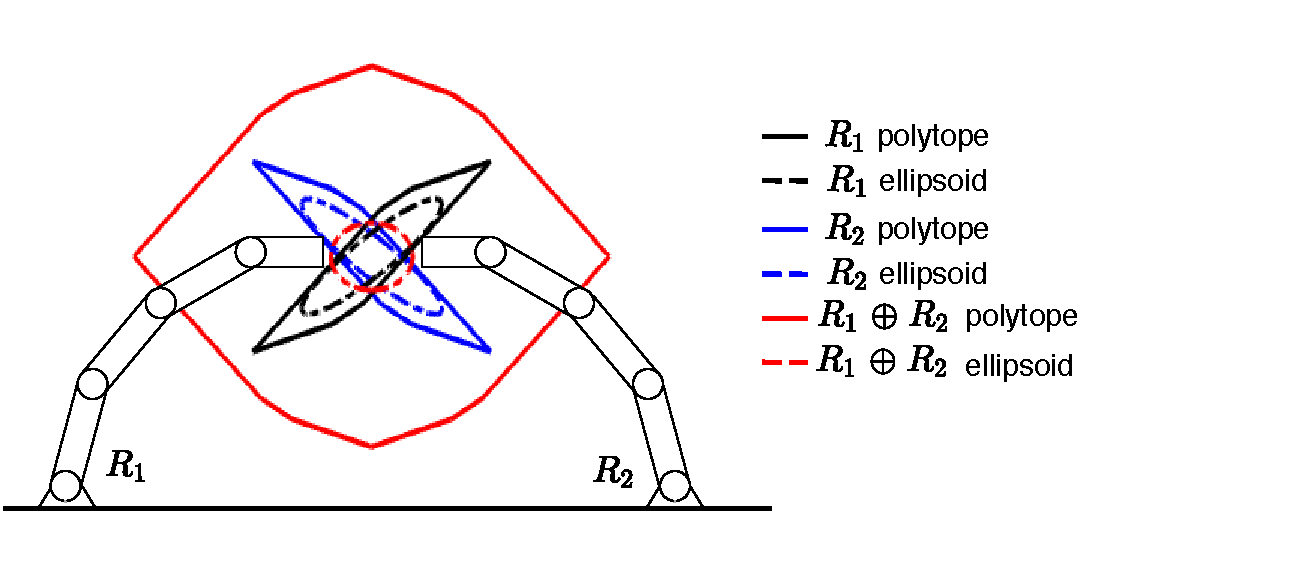
\includegraphics[width=\linewidth]{Papers/images/collaborative_difference.pdf}
    \caption{4DoF planar robots collaboration: polytopes and ellipsoids. Link lengths $l_i$$=$$0.5$, torque limit $|\tau_i|$$<$$1$ and joint angles $q_i$$=$$-\pi/8$ for $R_1$ and $q_i$$=$$\pi/8$ for $R_2$.}
    \label{fig:collaborative_difference}
\end{figure}

Up to recently \cite{long2020constrained}, the estimation of task-space capabilities of multiple robotic manipulators was largely depending on manipulability ellipsoids \cite{chiacchio_task_1991}\cite{chiacchio_global_1991}\cite{lee_dual_1989}.

However as the number of robots grows, the ellipsoid approach, which rely on a Euclidean norm rather than an infinity norm \cite{merlet_jacobian_2006}, provides a less accurate approximation and the question of what is the best practice to sum \cite{chiacchio_task_1991}\cite{julio_frantz_analysis_2015} or intersect \cite{sekiguchi_force_2017}\cite{lee_dual_1989} multiple ellipsoids becomes problematic. 

Figure \ref{fig:collaborative_difference} shows one example of two collaborating 4DoF planar robots joint force capacity based on ellipsoids and polytopes.  The ellipsoids are calculated using the approach proposed by Chiacchio \cite{chiacchio_task_1991} and the joint polytope is calculated as the Minkowski sum of the individual force polytope of each robot.
\begin{equation}
\mathcal{P}_{f_\oplus} = \mathcal{P}_{f_{R_1}} \oplus \mathcal{P}_{f_{R_2}} 
\end{equation}
This example clearly demonstrates that even though ellipsoids can reasonably well provide an approximation of the force capacity of each robot separately, the same is not the case for the capacity of the dyad.

A similar conclusion can be drawn for use cases where the joint capacity of multiple robots can be represented by the intersection of their polytopes \cite{long2020constrained}, \texit{i.e} when the robots are working in opposition, both applying a similar force $\bm{f}$ in opposite directions\footnote{A typical example of this situation is the case of the frictional grasp of an object.}
\begin{equation}
\mathcal{P}_f = \mathcal{P}_{f_{R_1}}  \cap \mathcal{P}_{f_{R_2}}     
\end{equation}
In that case, the polytope intersection problem can be elegantly transformed into the vertex enumeration problem for the extended system
\begin{equation}
J_\cap = [J_{R_1}\, J_{R_2}],\quad \bm{\tau} = \left[\bm{\tau}_{R_1}^T\, \bm{\tau}_{R_2}^T\right]^T, \quad J_\cap^T\bm{f} = \bm{\tau}
\end{equation}

\subsection{Polytopes for human-robot collaboration}
Several authors have studied the use of robotics performance measures such as manipulability ellipsoids and polytopes for human arms using 7DoF manipulator models \cite{rezzoug_application_2012}\cite{lazinica_higher_2010}\cite{carmichael_estimating_2013}\cite{carmichael_towards_2011} or full musculoskeletal model \cite{hernandez_toward_2015}. A promising approach for leveraging the efficient on-line polytope evaluation algorithm is to estimate the joint capacity of the robot and human and adapt the robotic assistance as a function of the evolution of human capabilities.  One of the associated challenges is to extend the proposed vertex search algorithms to actuation constraints which result from more complex actuation mechanisms such as muscles and can thus no longer be represented as parallelotopes.

\section{Conclusion}

The proposed vertex search algorithm provides a computationally efficient tool for the polytope-based, online evaluation of task-space robot capabilities. As illustrated in this work, the ability to accurately evaluate on-line the capabilities of robots leverages several possibilities in modern robotic applications where oversizing robots is no longer an option.




% \section{Conclusion}
% In this paper we presented a new real-time capable polytope vertex finding algorithm for efficient calculating twist and wrench polytopes. The new algorithm is capable of calculating polytope vertices for 6DOF and 7DOF robots under 3ms. An experimental setup with two collaborating \textit{Franka Amika Panda} robots has been created to demonstrate the algoritm potential. By leveraging the real force capacity evaluation we created a simple control strategy to safely carry the mass of 12 kilograms.
